% Phase 1 report: baseline reproduction of SeqCRC (Andeol et al., 2025). Build: tectonic report.tex (or pdflatex).
\documentclass[10pt]{article}
\usepackage[margin=0.6in,top=0.5in,bottom=0.55in]{geometry}
\usepackage[T1]{fontenc}
\usepackage{lmodern}
\usepackage{microtype}
\usepackage{amsmath}
\usepackage{booktabs,multirow,array,tabularx}
\usepackage{graphicx}
\usepackage{xcolor}
\usepackage[hidelinks]{hyperref}
\usepackage{enumitem}
\setlist{nosep,leftmargin=*}
\usepackage{caption}
\captionsetup{font=small,labelfont=bf,skip=3pt}
\setlength{\parskip}{2pt}
\setlength{\parindent}{0pt}
\usepackage{titlesec}
\titlespacing*{\section}{0pt}{5pt}{2pt}
\titleformat*{\section}{\normalsize\bfseries}
% The public GitHub repository of this reproduction.
\newcommand{\repourl}{\url{https://github.com/nicholas55555/seqcrc-baseline}}


\begin{document}
\begin{center}
{\large\bfseries Phase 1 Baseline Reproduction: Conformal Object Detection by Sequential Risk Control}\\[1pt]
Nicholas Taylor \;$\cdot$\; CAI 6930 Autonomous Vehicles \;$\cdot$\; Weather Adaptive Autonomous Driving \;$\cdot$\; Oct.\ 15, 2026
\end{center}
\vspace{-6pt}
\textbf{Paper reproduced.} L.~And\'eol, L.~Mossina, A.~Mazoyer, S.~Gerchinovitz, ``Conformal Object Detection by
Sequential Risk Control,'' arXiv:2505.24038, v2, Oct.\ 2025 (preprint; no peer-reviewed version yet).\\
\textbf{Original code:} \url{https://github.com/leoandeol/cods} (official; commit \texttt{269ff11}).
\textbf{Our repository:} \repourl.\\
Our project calibrates a frozen detector's confidence threshold per weather condition with SeqCRC's first step, so
the baseline is SeqCRC on its own benchmark: a COCO-pretrained YOLOv8x calibrated on MS-COCO. SeqCRC trains nothing;
its ``training'' is calibration of three scalars on 2,500 images, and evaluation is on the other 2,500.

\section{Setup}
\begin{itemize}
\item \textbf{GPU platform.} A local laptop instead of the online GPU the assignment asks for: NVIDIA GeForce RTX 3050 Ti Laptop GPU (4\,GB,
driver 566.07, CUDA 12.7), AMD Ryzen 7 4800H (8 cores), 32\,GB RAM, Windows 11. Detection ran on the GPU; calibration
ran on the CPU (Sec.~4, issue 4). The GPU is needed only for the one-off 390\,s detection pass (\texttt{logs/08}), which a
4\,GB card handles; we did not run the pipeline on a hosted GPU.
\item \textbf{Software.} Python 3.11.15 (uv), PyTorch 2.14.1 + torchvision 0.29.1 (CUDA 12.6 wheels), Ultralytics
8.4.177, NumPy 2.4.6, numba 0.68.0, pycocotools 2.0.11, scikit-learn 1.9.1; cods 0.4 at commit \texttt{269ff11} plus
our patch (repository \texttt{patches/}). Exact versions: \texttt{requirements.txt}.
\item \textbf{Data.} Full MS-COCO val2017 (5,000 images, SHA-256-checked); first 2,500 images for calibration,
last 2,500 for test, which is the official code's unshuffled 50/50 split.
\item \textbf{Protocol (paper, Sec.~V-A).} YOLOv8x (the official \texttt{yolov8x.pt} at Ultralytics' default 640\,px; the
paper states neither), NMS IoU 0.5, confidence floor
$10^{-3}$, $\alpha_{\text{tot}}=0.1$ split as $(\alpha_{\text{cnf}},\alpha_{\text{loc}},\alpha_{\text{cls}})=(0.02,0.05,0.05)$,
mix-matching weight $\tau=0.25$. The paper's appendix (Table VII) reports 92 YOLOv8x combinations at this budget; we ran four of
them in full (F1--F4), chosen to cover both confidence losses, the Hausdorff, LAC and Mix matchings, pixel-wise and
box-wise localization losses, additive and multiplicative boxes, and APS and LAC class sets.
\end{itemize}

\section{Results}
\begin{table}[h]
\centering\footnotesize
\setlength{\tabcolsep}{3.2pt}
\caption{SeqCRC with YOLOv8x on COCO val2017, $\alpha_{\text{tot}}=0.1$: set size and test risk per task (confidence:
boxes per image, budget 0.02; localization: box stretch, 0.05; classification: classes per set, 0.05) and global risk
(budget 0.1). Paper: App.\ Table VII. Full: the same 2{,}500/2{,}500 split. 300/300: first 300 calibration, next 300 test.}
\label{tab:seqcrc}
\begin{tabular}{@{}l p{3.3cm} l rr rr rr r@{}}
\toprule
 & Matching / conf.\ loss / loc.\ loss-set / class set & Source & \multicolumn{2}{c}{Confidence} & \multicolumn{2}{c}{Localization} & \multicolumn{2}{c}{Classification} & Global \\
\cmidrule(lr){4-5}\cmidrule(lr){6-7}\cmidrule(lr){8-9}
 & & & size & risk & size & risk & size & risk & risk \\
\midrule
\multirow{3}{*}{F1} & \multirow{3}{*}{\parbox{3.3cm}{\raggedright Hausdorff / bc-recall / pixel-add / APS}} & Paper & 11.71 & 0.019 & 3.87 & 0.049 & 41.73 & 0.043 & 0.082 \\
 &  & Ours, full & 11.53 & 0.020 & 1.30 & 0.053 & 40.64 & 0.042 & 0.085 \\
 &  & Ours, 300/300 & 11.11 & 0.025 & 1.30 & 0.040 & 42.67 & 0.033 & 0.066 \\
\addlinespace[3pt]
\multirow{3}{*}{F2} & \multirow{3}{*}{\parbox{3.3cm}{\raggedright LAC / bc-thresh / pixel-add / LAC}} & Paper & 18.86 & 0.012 & 20.64 & 0.047 & 0.72 & 0.049 & 0.086 \\
 &  & Ours, full & 18.02 & 0.015 & 17.69 & 0.047 & 0.75 & 0.046 & 0.083 \\
 &  & Ours, 300/300 & 14.29 & 0.047 & 13.56 & 0.046 & 1.02 & 0.045 & 0.080 \\
\addlinespace[3pt]
\multirow{3}{*}{F3} & \multirow{3}{*}{\parbox{3.3cm}{\raggedright Mix / bc-recall / pixel-mult / LAC}} & Paper & 11.71 & 0.019 & 4.54 & 0.049 & 67.58 & 0.053 & 0.098 \\
 &  & Ours, full & 11.53 & 0.020 & 1.24 & 0.052 & 66.82 & 0.055 & 0.100 \\
 &  & Ours, 300/300 & 11.11 & 0.025 & 1.24 & 0.038 & 66.06 & 0.061 & 0.093 \\
\addlinespace[3pt]
\multirow{3}{*}{F4} & \multirow{3}{*}{\parbox{3.3cm}{\raggedright Mix / bc-thresh / box-add / APS}} & Paper & 18.86 & 0.012 & 6.12 & 0.043 & 40.75 & 0.042 & 0.078 \\
 &  & Ours, full & 18.02 & 0.015 & 2.56 & 0.053 & 38.28 & 0.043 & 0.088 \\
 &  & Ours, 300/300 & 14.29 & 0.047 & 2.21 & 0.055 & 40.66 & 0.038 & 0.085 \\
\bottomrule
\end{tabular}
\end{table}

\begin{table}[h]
\centering\footnotesize
\caption{Detector check: COCO box AP of YOLOv8x on all 5{,}000 val2017 images (pycocotools).}
\label{tab:det}
\begin{tabular}{@{}lrrr@{}}
\toprule
Boxes scored & AP & AP50 & AP75 \\
\midrule
Ultralytics model table (paper's detector) & 53.9 & -- & -- \\
Ours: Ultralytics predict, NMS IoU 0.7 per class & 53.2 & 69.8 & 58.0 \\
Ours: Ultralytics predict, class-agnostic NMS IoU 0.5 & 51.6 & 68.8 & 55.6 \\
Ours: cods YOLO wrapper, batch 1 (SeqCRC input) & 45.1 & 65.9 & 48.2 \\
Ours: cods YOLO wrapper, batch 8 & 10.7 & 32.1 & 1.4 \\
\bottomrule
\end{tabular}
\end{table}



On the full 2{,}500/2{,}500 split the confidence and classification steps reproduce closely: the box-count-recall
step keeps 11.53 boxes per image in F1 and F3 (paper 11.71) and the box-count-threshold step 18.02 in F2 and F4 (paper
18.86), and the class sets hold 40.6, 0.75, 66.8 and 38.3 classes in F1--F4 (paper 41.7, 0.72, 67.6 and 40.8). Test
risks sit at or near their budgets, as in the paper: global risks are 0.085, 0.083, 0.0997 and 0.088 against the 0.1
budget (paper 0.082, 0.086, 0.098 and 0.078), and a few single-split task risks are slightly above theirs (at most
0.055 against 0.05), as is the paper's own F3 classification risk (0.053; see the sampling-noise item in
Sec.~\ref{sec:disc}). Localization is the exception: our stretches are smaller in every configuration (F1: 1.31
against 3.87; F3: 1.24 against 4.54; F4: 2.56 against 6.12), which Sec.~\ref{sec:disc} traces to the batch size.

\small
\section{Discrepancies}\label{sec:disc}
\begin{itemize}
\item \textbf{Localization sets are much smaller than reported for YOLOv8x; class sets and box-count-recall confidence
sets are close.}
The likely cause is in the official YOLO wrapper (\texttt{cods/od/models/yolo.py}): it rescales the raw head output by
original/letterboxed image size and never removes the letterbox padding. With batch size 1 (our runs) Ultralytics pads
each image only to a multiple of 32, so the error is small; with a batch of differently sized images it pads every
image to $640\times640$ and the boxes land far from the objects. Table~\ref{tab:det} shows the effect directly: the
same wrapper scores 45.1 AP at batch 1 but 10.7 AP (AP75 1.4) at batch 8. Re-running F3 on the 300/300 subset with batch 8 raises
the stretch from 1.24 to 4.70, close to the paper's 4.54, while the confidence and class sets barely move (11.11 vs.\
11.46 boxes, 66.1 vs.\ 65.7 classes). The paper's best YOLOv8x stretches (3.87--5.45, its Table III) are also 3--4
times those of DETR-101 (1.04--1.55), whose wrapper rescales normalized boxes and is unaffected. The paper does not state
its batch size, but the official tutorial notebook calls \texttt{build\_predictions} with \texttt{batch\_size=12} next to a
commented-out \texttt{YOLOModel("yolov8x.pt")} line, so its YOLOv8x localization numbers were most likely produced with a
batch size above 1. (One configuration on 300/300 images; a full-size batch-8 run did not finish in time.)
\item \textbf{The detector itself reproduces.} Through Ultralytics we measure 53.2 AP against the published 53.9 (we use
\texttt{predict()} with per-image letterboxing and pycocotools, not \texttt{val()}). The boxes SeqCRC actually
receives score 45.1: class-agnostic NMS at IoU 0.5 (the paper's IoU; the cods NMS is class-agnostic) costs 1.6 AP (51.6), and the wrapper's
box rescaling (padding not removed, separate $x$/$y$ scales, no clipping) costs the remaining 6.5; its scores and classes
are the same maximum sigmoid score and argmax that Ultralytics uses. We kept the official wrapper because it is what the paper's numbers come from.
\item \textbf{One split, sampling noise.} The paper reports a single calibration/test draw, as we do; the guarantee is on
the expectation over draws, so single-split risks may sit slightly above or below the budget. On 300 test images the
fluctuations are larger (e.g., box-count-threshold risk 0.047 against 0.02).
\item \textbf{Software drift.} We ran the code at HEAD \texttt{269ff11} (22 May 2026; library code last changed 22 Oct
2025) with Ultralytics 8.4.177; the paper's runs used
earlier versions (not stated). Our two speed patches changed no output: the mask selection is exact, and the float64 running
sum moved calibration risks by about $2\times10^{-9}$, leaving every output of a 300/300 check identical (Sec.~4).
\end{itemize}

\section{Issues and fixes}
\begin{enumerate}
\item \textbf{Hard-coded path and logging.} \texttt{cods/od/evaluate.py} reads COCO from
\texttt{/datasets/shared\_datasets/coco/} and requires Weights \& Biases. \emph{Fix:} \texttt{scripts/run\_seqcrc.py}
repeats its \texttt{run\_experiment} step for step with a \texttt{-{}-coco} argument and JSON-lines output, and adds the
paper's $10^{-3}$ floor, which \texttt{evaluate.py} never applies (the tutorial notebook uses $4\times10^{-2}$).
\item \textbf{Calibration crashes at HEAD} (\texttt{TypeError: expected Tensor \dots\ but got list}). Lint commit
\texttt{e70d773} (20 Oct 2025) turned \texttt{x = list([\dots],)} into \texttt{x = ([\dots],)} in
\texttt{build\_predictions}, wrapping every per-image list in a 1-tuple; the tutorial notebook only works from older
cached predictions. \emph{Fix:} unwrap the tuples when \texttt{ODPredictions} is built (no upstream edit).
\item \textbf{4\,GB GPU and device mismatch.} Unfiltered YOLOv8x outputs (hundreds of boxes per image, each with a
91-way class vector) do not fit, and ground truth and boxes ended up on different devices. \emph{Fix:} apply the
paper's $10^{-3}$ floor right after NMS (the same box set), keep boxes on the CPU, then move all predictions to one
device; this leaves 50.8 boxes per test image on average (median 30, max 741).
\item \textbf{Calibration too slow for a laptop.} A 50/50-image smoke test was still calibrating after about 12\,min on
the GPU and was killed (\texttt{logs/02}); profiling with \texttt{py-spy} pointed to (a) a
Python loop over every box for every candidate threshold and (b) a full re-summation of all $n$ per-image losses after
each single update, $O(n^2)$ overall (100 images: 294\,s; 300: 1,151\,s; extrapolated to 2,500: $\approx$8\,h per
configuration). \emph{Fix} (\texttt{patches/cods-reproduction.patch}): boolean-mask indexing, which selects the same
rows in the same order, and a running sum of the losses. Unit tests show identical selections and sums (within
$10^{-6}$), and a 300/300 run with and without the running sum gives the same step-1 thresholds to every printed
digit. Calibration then runs on the CPU,
one thread per process; the four full runs ran in parallel, with diagnostic runs alongside, so their wall-clock times
were measured under CPU contention.
\item \textbf{Smaller snags.} With 10 calibration images cods reports ``No good lambda found'', correctly: SeqCRC
needs $\alpha_{\text{loc}}\ge\alpha_{\text{cnf}}+1/(n+1)$, so smoke tests use $n\ge100$. On Windows, \texttt{python}
was the Microsoft Store stub and console output failed on \texttt{cp1252}; we used a uv-managed CPython and
\texttt{PYTHONIOENCODING=utf-8}.
\end{enumerate}

\normalsize
\section{Evidence}
\noindent\begin{minipage}[t]{0.565\linewidth}\vspace{0pt}
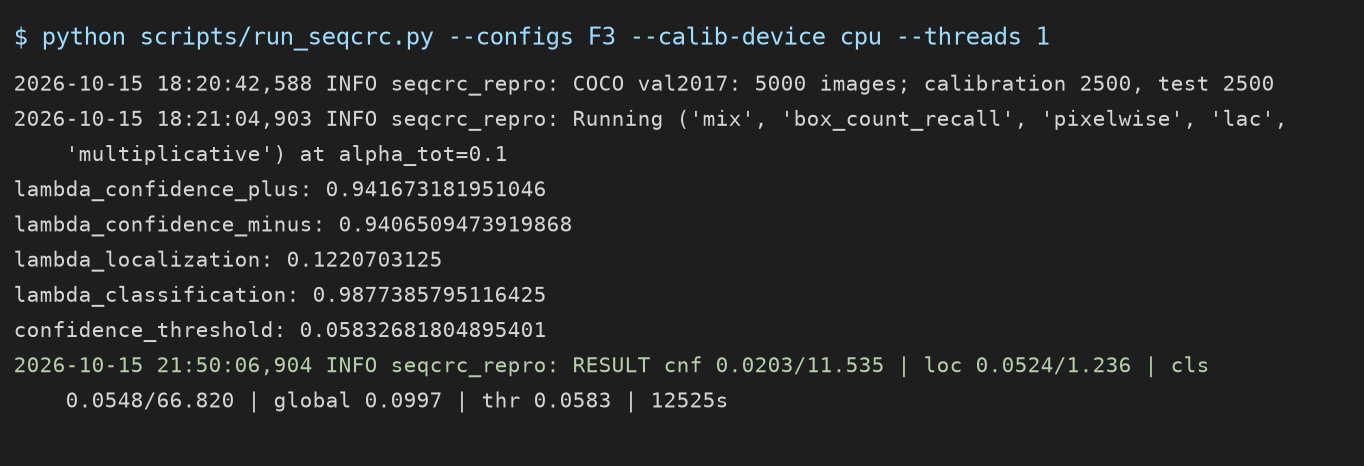
\includegraphics[width=\linewidth]{fig_evidence_run.png}
\end{minipage}\hfill
\begin{minipage}[t]{0.42\linewidth}\vspace{0pt}
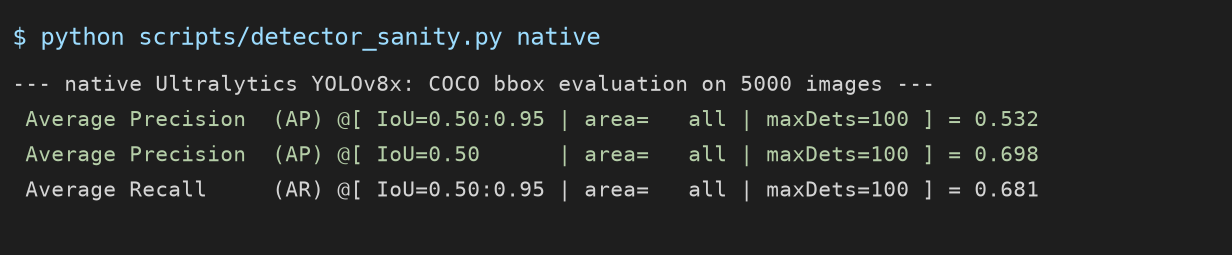
\includegraphics[width=\linewidth]{fig_evidence_detector.png}\\[3pt]
{\footnotesize Fig.~1. Excerpts of the saved logs (lines selected and wrapped, text unchanged; the first line names the
command). Left: a full-size SeqCRC run (\texttt{RUN_LOG_NAME}). Right: COCO evaluation of YOLOv8x
(\texttt{logs/11\_detector\_sanity\_native.log}).\par}
\end{minipage}

\end{document}
